%%%%%%%%%%%%%%%%%%%%%%%%%%%%%%%%%%%%%%%%%
% University/School Laboratory Report
% LaTeX Template
% Version 4.0 (March 21, 2022)
%
% This template originates from:
% https://www.LaTeXTemplates.com
%
% Authors:
% Vel (vel@latextemplates.com)
% Linux and Unix Users Group at Virginia Tech Wiki
%
% License:
% CC BY-NC-SA 4.0 (https://creativecommons.org/licenses/by-nc-sa/4.0/)
%
%%%%%%%%%%%%%%%%%%%%%%%%%%%%%%%%%%%%%%%%%

%----------------------------------------------------------------------------------------
%	PACKAGES AND DOCUMENT CONFIGURATIONS
%----------------------------------------------------------------------------------------

\documentclass[
	letterpaper, % Paper size, specify a4paper (A4) or letterpaper (US letter)
	10pt, % Default font size, specify 10pt, 11pt or 12pt
]{CSUniSchoolLabReport}

%----------------------------------------------------------------------------------------
%	REPORT INFORMATION
%----------------------------------------------------------------------------------------

\title{ECE 398-MA \\ Introduction to Modern Communication with Python and SDR \\ Lab 5 -- Pulse-Shaping} % Report title

\author{Noah Breit} % Author name(s), add additional authors like: '\& James \textsc{Smith}'

\date{\today} % Date of the report

%----------------------------------------------------------------------------------------

\begin{document}

\maketitle % Insert the title, author and date using the information specified above

% \begin{center}
% 	\begin{tabular}{l r}
% 		Date Performed: & February 13, 2022 \\ % Date the experiment was performed
% 		Partners: & Cecilia \textsc{Smith} \\ % Partner names
% 		& Tajel \textsc{Khumalo} \\
% 		Instructor: & Professor \textsc{Rivera} % Instructor/supervisor
% 	\end{tabular}
% \end{center}

% If you need to include an abstract, uncomment the lines below
%\begin{abstract}
%	Abstract text
%\end{abstract}

%----------------------------------------------------------------------------------------
%	OBJECTIVE
%----------------------------------------------------------------------------------------

\section{Assignment 1}

\begin{lstlisting}[language=Python]
	import numpy as np
	import matplotlib.pyplot as plt
	
	num_symbols = 64
	sps = 16
	
	############# PART 1 ##############
	def generate_bpsk_symbols(num_symbols):
	"""Generate BPSK symbols from random bits."""
	np.random.seed(0)
	bits = np.random.randint(0, 2, num_symbols)
	symbols = np.where(bits == 1, 1, -1)
	return symbols
	
	def upsample_symbols(symbols, sps):
	"""Upsample symbols by inserting zeros."""
	up_sym = np.zeros(len(symbols) * sps)
	up_sym[::sps] = symbols
	return up_sym
	
	def plot_upsampled_symbols(up_sym):
	"""Plot upsampled symbols."""
	plt.figure()
	plt.stem(up_sym)
	plt.title("Upsampled Symbols")
	plt.show()
	
	# part 1 driver
	symbols = generate_bpsk_symbols(num_symbols)
	up_sym = upsample_symbols(symbols, sps)
	plot_upsampled_symbols(up_sym)
	
\end{lstlisting}

\begin{figure}[H] % [H] forces the figure to be placed exactly where it appears in the text
	\centering % Horizontally center the figure
	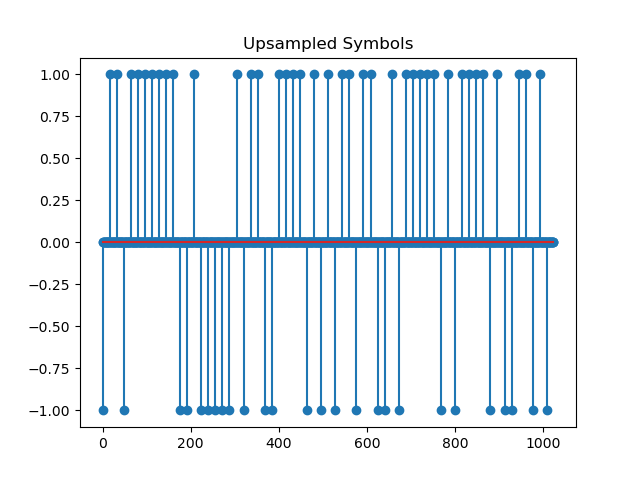
\includegraphics[width=1.2\textwidth]{assignment1.png} % Include the figure
	\caption{Upsampled BPSK Symbols}
	\label{fig:block}
\end{figure}

\section{Assignment 2}

\begin{lstlisting}[language=Python]
	############ PART 2 ################
	def rcosfilter(N, alpha, Tb, Fs):
	"""
	Generates a raised cosine (RC) filter (FIR) impulse response.
	
	Parameters
	----------
	N : int
	Length of the filter in samples.  
	
	alpha : float
	Roll off factor (Valid values are [0, 1]).
	
	Tb : float
	Symbol period.
	
	Fs : float
	Sampling Rate.
	
	Returns
	---------
	h_rc : 1-D ndarray of floats
	Impulse response of the raised cosine filter.
	"""
	t = ((np.arange(N) - N / 2))*1/float(Fs)
	h_rc = np.sinc(t / Tb) * np.cos(np.pi * alpha * t / Tb) / (1 - 4 * alpha**2 * t**2 / Tb**2)
	# h_rc[np.abs(t) > Tb / (2 * alpha)] = 0  # Ensure filter is zero outside the main lobe
	return h_rc
	
	def rectangular_pulse(N):
	"""Generate rectangular pulse."""
	return np.ones(N)
	
	def convolve_with_pulse(up_sym, pulse):
	"""Convolve upsampled symbols with a pulse."""
	return np.convolve(up_sym, pulse, mode='full')
	
	def plot_time_domain(x):
	"""Plot signal in time domain."""
	plt.figure()
	plt.plot(x)
	plt.title("Time Domain")
	plt.show()
	
	def plot_frequency_domain(x):
	"""Plot signal in frequency domain."""
	plt.figure()
	plt.plot(np.abs(np.fft.fft(x)))
	plt.yscale('log')
	plt.title("Frequency Domain")
	plt.show()
	
	def plot_eye_diagram(x, sps, numeye=2):
	"""Plot eye diagram."""
	plt.figure()
	for k in range(len(x) // sps):
	start_idx = k * sps - sps // 2
	end_idx = (k + numeye) * sps + sps // 2
	if start_idx < 0:
	start_idx = 0
	if end_idx > len(x):
	break
	plt.plot(x[start_idx:end_idx], color='gray', alpha=0.5, linewidth=1.5)
	plt.xlabel('Time')
	plt.ylabel('Amplitude')
	plt.grid(True)
	plt.show()
	
	# part 2 driver
	N = 15 * sps + 1
	Tb = sps
	Fs = 1
	
	# Rectangular Pulse
	rect_pulse = rectangular_pulse(sps)
	rect_convolved = convolve_with_pulse(up_sym, rect_pulse)
	plot_time_domain(rect_convolved)
	plot_frequency_domain(rect_convolved)
	plot_eye_diagram(rect_convolved, sps)
	
	# Raised-cosine Pulses
	alphas = [0, 0.5, 1]
	for alpha in alphas:
	rc_pulse = rcosfilter(N, alpha, Tb, Fs)
	rc_convolved = convolve_with_pulse(up_sym, rc_pulse)
	plot_time_domain(rc_convolved)
	plot_frequency_domain(rc_convolved)
	plot_eye_diagram(rc_convolved, sps)

\end{lstlisting}

\begin{figure}[H] % [H] forces the figure to be placed exactly where it appears in the text
	\centering % Horizontally center the figure
	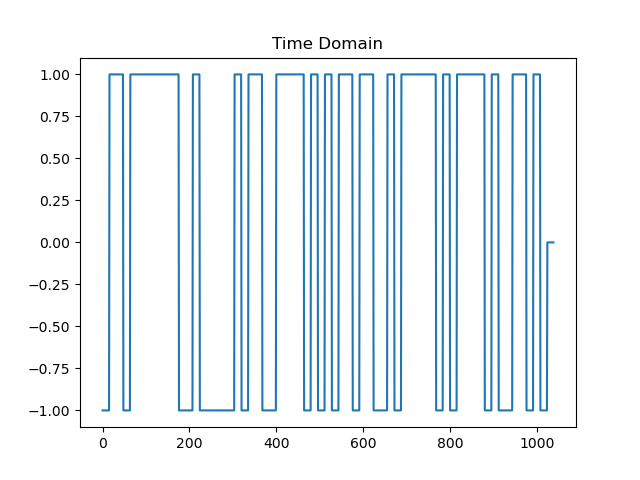
\includegraphics[width=1.2\textwidth]{assignment2a.png} % Include the figure
	\caption{Rect Pulse -- Time-Domain Signal}
	\label{fig:block}
\end{figure}

\begin{figure}[H] % [H] forces the figure to be placed exactly where it appears in the text
	\centering % Horizontally center the figure
	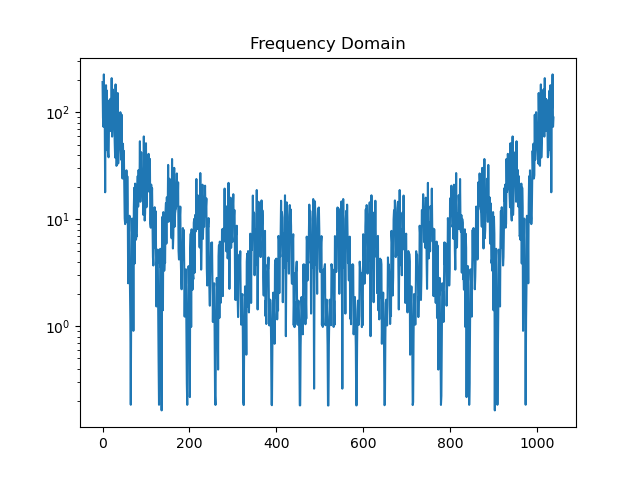
\includegraphics[width=1.2\textwidth]{assignment2b.png} % Include the figure
	\caption{Rect Pulse -- Freq-Domain Signal}
	\label{fig:block}
\end{figure}

\begin{figure}[H] % [H] forces the figure to be placed exactly where it appears in the text
	\centering % Horizontally center the figure
	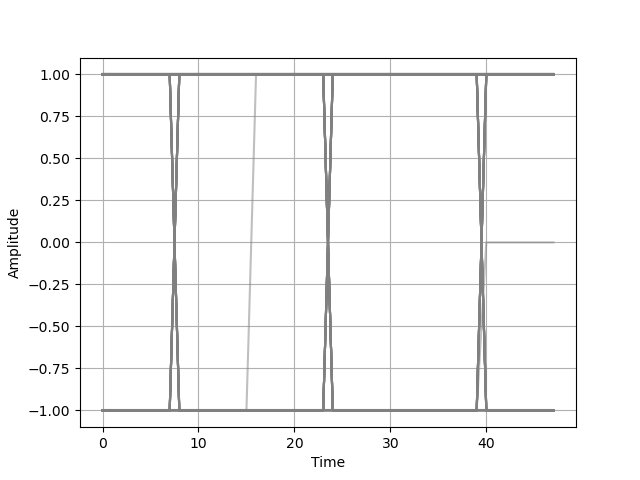
\includegraphics[width=1.2\textwidth]{assignment2c.png} % Include the figure
	\caption{Rect Pulse -- Eye Diagram}
	\label{fig:block}
\end{figure}

\begin{figure}[H] % [H] forces the figure to be placed exactly where it appears in the text
	\centering % Horizontally center the figure
	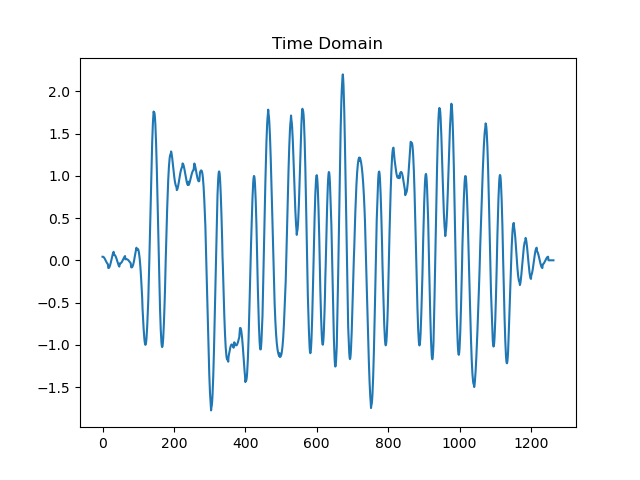
\includegraphics[width=1.2\textwidth]{assignment2d.png} % Include the figure
	\caption{Cosine Pulse ALPHA=0 -- Time-Domain Signal}
	\label{fig:block}
\end{figure}

\begin{figure}[H] % [H] forces the figure to be placed exactly where it appears in the text
	\centering % Horizontally center the figure
	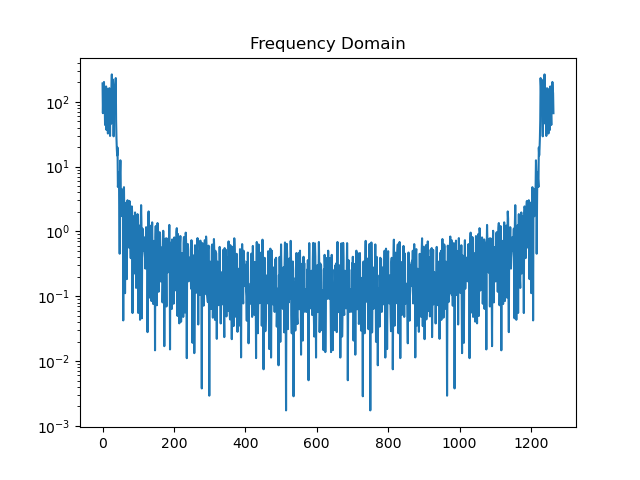
\includegraphics[width=1.2\textwidth]{assignment2e.png} % Include the figure
	\caption{Cosine Pulse ALPHA=0 -- Freq-Domain Signal}
	\label{fig:block}
\end{figure}

\begin{figure}[H] % [H] forces the figure to be placed exactly where it appears in the text
	\centering % Horizontally center the figure
	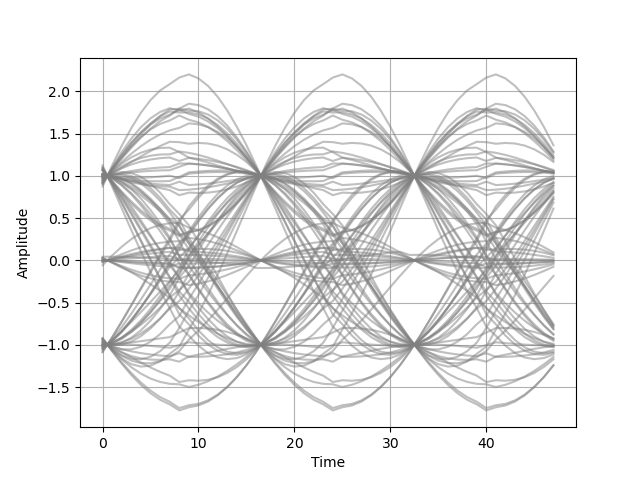
\includegraphics[width=1.2\textwidth]{assignment2f.png} % Include the figure
	\caption{Cosine Pulse ALPHA=0 -- Eye Diagram}
	\label{fig:block}
\end{figure}

\begin{figure}[H] % [H] forces the figure to be placed exactly where it appears in the text
	\centering % Horizontally center the figure
	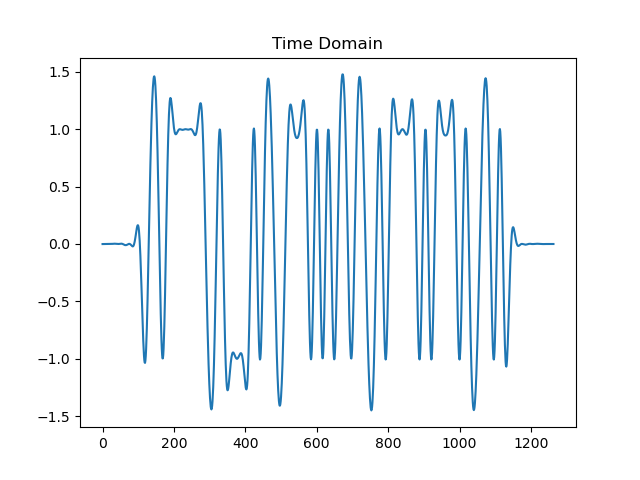
\includegraphics[width=1.2\textwidth]{assignment2g.png} % Include the figure
	\caption{Cosine Pulse ALPHA=0.5 -- Time-Domain Signal}
	\label{fig:block}
\end{figure}

\begin{figure}[H] % [H] forces the figure to be placed exactly where it appears in the text
	\centering % Horizontally center the figure
	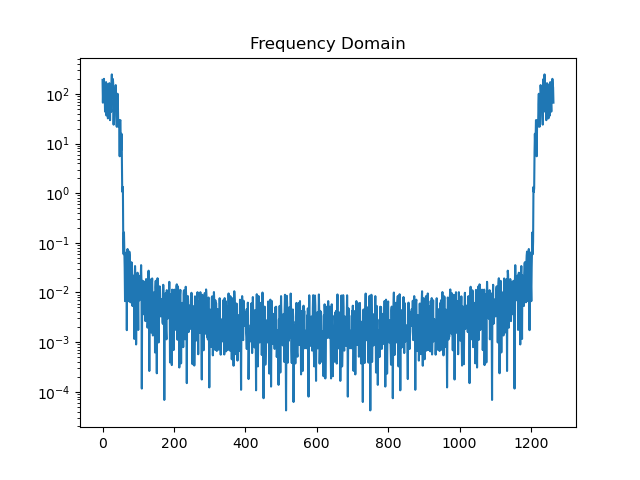
\includegraphics[width=1.2\textwidth]{assignment2h.png} % Include the figure
	\caption{Cosine Pulse ALPHA=0.5 -- Freq-Domain Signal}
	\label{fig:block}
\end{figure}

\begin{figure}[H] % [H] forces the figure to be placed exactly where it appears in the text
	\centering % Horizontally center the figure
	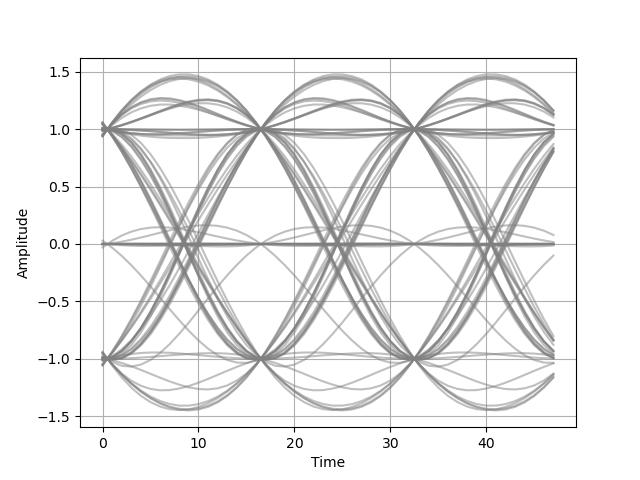
\includegraphics[width=1.2\textwidth]{assignment2i.png} % Include the figure
	\caption{Cosine Pulse ALPHA=0.5 -- Eye Diagram}
	\label{fig:block}
\end{figure}

\begin{figure}[H] % [H] forces the figure to be placed exactly where it appears in the text
	\centering % Horizontally center the figure
	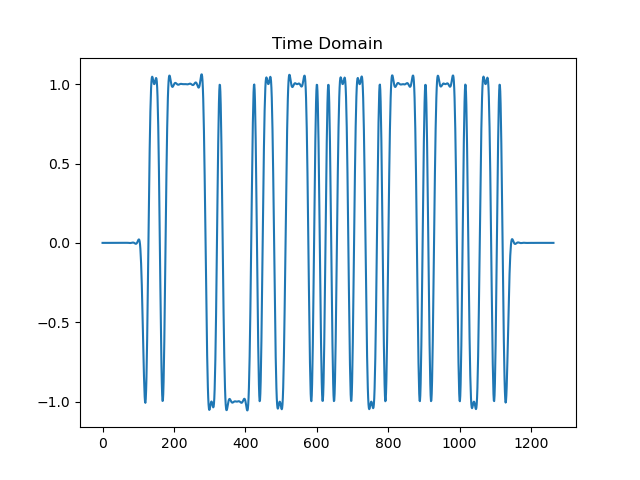
\includegraphics[width=1.2\textwidth]{assignment2j.png} % Include the figure
	\caption{Cosine Pulse ALPHA=1 -- Time-Domain Signal}
	\label{fig:block}
\end{figure}

\begin{figure}[H] % [H] forces the figure to be placed exactly where it appears in the text
	\centering % Horizontally center the figure
	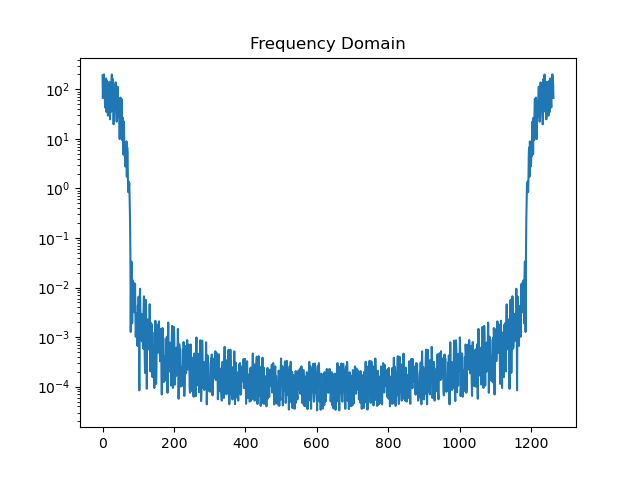
\includegraphics[width=1.2\textwidth]{assignment2k.png} % Include the figure
	\caption{Cosine Pulse ALPHA=1 -- Freq-Domain Signal}
	\label{fig:block}
\end{figure}

\begin{figure}[H] % [H] forces the figure to be placed exactly where it appears in the text
	\centering % Horizontally center the figure
	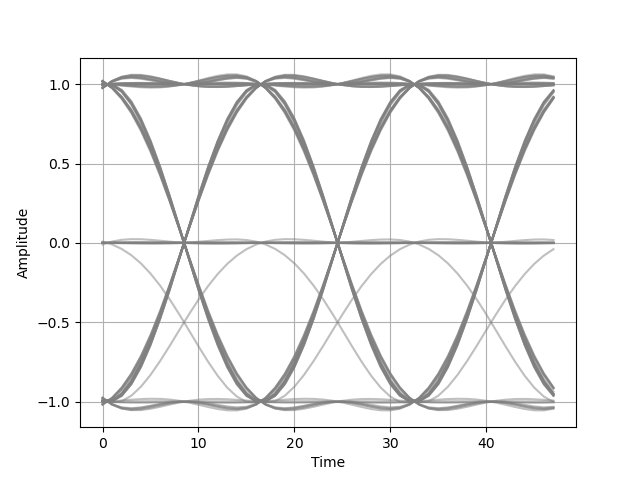
\includegraphics[width=1.2\textwidth]{assignment2m.png} % Include the figure
	\caption{Cosine Pulse ALPHA=1 -- Eye Diagram}
	\label{fig:block}
\end{figure}

\end{document}